\documentclass[11pt,letter]{article}

\usepackage[latin1]{inputenc}
\usepackage{amsmath}
\usepackage{amsfonts}
\usepackage{amssymb}
\usepackage{amsthm}
\usepackage{enumitem}
\usepackage[english]{babel}
\usepackage{fancyhdr}
\usepackage{lipsum}
\usepackage{chngpage}
\usepackage{geometry}
\usepackage{mathtools}
\usepackage{tabularx}
\usepackage{verbatim}
\usepackage{tikz}
\usepackage[ruled,vlined]{algorithm2e}
\geometry{letterpaper, portrait, margin=1in}
 
\pagestyle{fancy}
\fancyhf{}
\rhead{\thepage}
\lhead{Implementing Path 3-Coloring and Path 3-Choosing Algorithms on Plane Graphs}
\rfoot{}

\newcommand{\overbar}[1]{\mkern 1.5mu\overline{\mkern-1.5mu#1\mkern-1.5mu}\mkern 1.5mu}

\begin{document}

\title{Implementing Path 3-Coloring and Path 3-Choosing Algorithms on Plane Graphs}
\date{August 2, 2016}

\maketitle

\section*{Abstract}

Path coloring a graph partitions its vertices into sets inducing a disjoint union of paths. In this project
we consider several algorithms to compute path colorings of graphs embedded in the plane. We
first implement an algorithm path 3-color plane graphs from Poh's proof in [a]. Second, we present a linear time
implementation of an algorithm to path 3-choose plane graphs from the independant work of Hartman [b] and
Skrekovski [c].

\section{Introduction}

All graphs discussed in this project will be simple, undirected, and finite. A graph is planar if it may
be drawn in the plane without edge crossings. A $k$-coloring of a graph partitions
its vertices into $k$ color classes. Such a coloring is called proper if each color class consists of
nonadjacent vertices.\\

\noindent In 1976 Appel and Haken [d,e] displayed that all planar graphs have a proper $4$-coloring.
This result is best possible and solved the century old Four Color Conjecture.
Generalizations of proper coloring were introduced in [f,g,h] allowing color classes to form forests, or allowing vertices
to have some bounded number of same color neighbors. Cowen et al. ([j]) show a best possible result that planar
graphs may be $3$-colored such that each vertex recieves at most two same color neighbors.\\

\noindent We will be considering the problem of path coloring, producing a $k$-coloring of a graph such that each color
class induces a disjoint union of paths, or equivalently a forest where each component is a path. This coloring
was introduced by Harary in [i]. Note that this is similar to the defective coloring of Cowen et al. above,
with the added restriction that path coloring forbids cycles. In [l] Poh displayes that all
planar graphs have a path $3$-coloring. Here we present an implementation of Poh's algorithm to path
$3$-color plane graphs.\\

\noindent Given a list of $k$ colors for each vertex, a $k$-list-coloring, or $k$-choosing, assigns each vertex a
color from its list.
If a graph has a proper $k$-choosing it is said to be $k$-choosable. List-coloring was first introduced by
Erd{\"o}s et al. in [m]. Thomassen in [n] proves that all planar graphs are $5$-choosable. Planar
graphs that are not $4$-choosable are described by Mirzakhani in [o] and Voigt in [p], so Thomassen's result
is best possible. Jensen and Toft in [t] note that Thomassen's proof yields a linear algorithm for $5$-choosing
plane graphs.\\

\noindent Hull and Eaton in [q] prove planar graphs are $3$-choosable such that each vertex recieves at most two
same color neighbors, and furthermore show this result is best possible. Hartman in [r] and Skrekovski in [s] independantly
provide similar proofs that planar graphs are path $3$-choosable. Hartman claims the proof yields
a linear time algorithm for path $3$-list-coloring, and thus path $3$-coloring, plane graphs. Here we present a
linear time implementation of Hartman and Skrekovski's algorithm.

\section{Path $3$-Coloring Plane Graphs}

We first restate the theorem and proof of Poh [l]. This proof yields a simple algorithm for path $3$-coloring
plane graphs.\\

\begin{adjustwidth}{1.5em}{1.5em}
\noindent\textbf{Theorem 1.} Let $G$ be a $2$-connected weakly triangulated plane graph or a complete
graph on two vertices and
suppose the outer face $C$ has been $2$-colored such that each color class induces a non-empty path. This
$2$-coloring may be extended to a path $3$-coloring of $G$ such that no vertex in $V(C)$ recieves a same color
neighbor in $V(G)\setminus V(C)$.\\
\end{adjustwidth}

\begin{proof}
\noindent If $|V(G)|\le 2$ the coloring follows trivially. Let $|V(G)|>2$ and suppose the theorem holds
for all graphs $H$ with $|V(H)|<|V(G)|$. Let $P=p_0\ldots p_n$ and $Q=q_0\ldots q_m$ denote the two induced paths from the $2$-coloring of $C$
such that the edges $p_0q_0$ and $p_nq_m$ are in $C$. Suppose there exist uncolored vertices, that is
$V(G)\setminus V(C)\ne\emptyset$.\\

\noindent Let $t_0$ be the vertex forming a face with $p_0$ and $q_0$. If $t_0\in P$, this face is already
colored and we consider the graph bounded by $P-p_0$ and $Q$. Similarly, if $t_0\in Q$ then the inductive
hypothesis applies to the graph bounded by $P$ and $Q-q_0$. Let $t_1$ be the vertex forming a face with $p_n$
and $q_m$ and proceed in the same manner until $t_1$ is not in either path.\\

\noindent Suppose there exists an induced path $T$ from $t_0$ to $t_1$. We color $T$ the remaining color not
assigned to $P$ or $Q$ and apply the inductive hypothesis to the subgraph bounded by $P$ and $T$, and the
subgraph bounded by $T$ and $Q$. With only the path $T$ in common between the two subgraphs, the combined
$3$-coloring forms a path coloring of $G$.\\

\noindent Suppose no such path exists from $t_0$ to $t_1$. Since $G$ is weakly triangulated there must exist an
edge $p_iq_j\in E(G)\setminus E(C)$ with $p_i\in P$ and $q_j\in Q$. We separately apply the inductive hypothesis
to the subgraph bounded by $p_0\ldots p_i$ and $q_0\ldots q_j$, and the subgraph bounded by $p_i\ldots p_n$ and
$q_j\ldots q_m$. The two subgraphs only share the vertices $p_i$ and $q_j$, thus the combined $3$-coloring forms
a path coloring of $G$.
\end{proof}

\subsection*{Implementing Poh's Algorithm}

Let the plane graph $G$ be represented as an incidence list (or adjacency list) and an ordering of edges around
each vertex following a
combinatorial embedding. We track the paths $P$ and $Q$ by marking each vertex with its respective path and
storing the path start and end vertices $p_0$, $p_n$, $q_0$, and $q_m$.
We first find $t_1$ by looking through the ordered neighbors of $q_m$ and take the vertex counterclockwise past
$p_n$. This step is repeated until the graph is colored or $t_1\not\in P\cup Q$.\\

\begin{center}
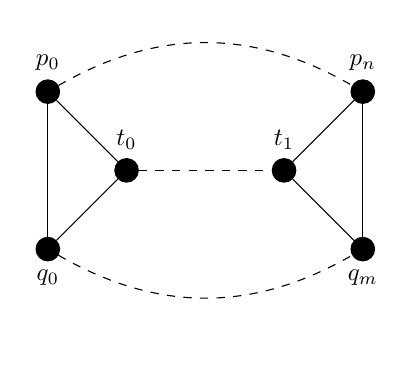
\begin{tikzpicture}[
		scale=1,
		every node/.style={circle, draw, minimum size=1mm, scale=0.9},
		every label/.append style={rectangle}
	]
  \node (p0) [label=above:$p_0$, fill] at (-2cm, 1cm) {};
  \node (pn) [label=above:$p_n$, fill] at (2cm, 1cm) {};
  \node (q0) [label=below:$q_0$, fill] at (-2cm, -1cm) {};
  \node (qn) [label=below:$q_m$, fill] at (2cm, -1cm) {};
  \node (t0) [label=above:$t_0$, fill] at (-1cm, 0cm) {};
  \node (t1) [label=above:$t_1$, fill] at (1cm, 0cm) {};
  \node (null) [draw=none] at (270:2cm) {};
  \draw (p0) edge [bend left] (pn) [dashed];
  \draw (q0) edge [bend right] (qn) [dashed];
  \draw (p0) edge (q0);
  \draw (pn) edge (qn);
  \draw (p0) edge (t0);
  \draw (q0) edge (t0);
  \draw (pn) edge (t1);
  \draw (qn) edge (t1);
  \draw (t0) edge (t1) [dashed];
\end{tikzpicture}
$\qquad$
\begin{tikzpicture}[
		scale=1,
		every node/.style={circle, draw, minimum size=1mm, scale=0.9},
		every label/.append style={rectangle}
	]
  \node (null) [draw=none] at (0cm, 0cm) {$\rightarrow$};
  \node (null) [draw=none] at (270:2cm) {};
\end{tikzpicture}
$\qquad$
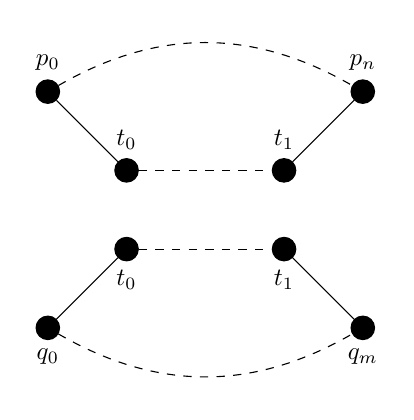
\begin{tikzpicture}[
		scale=1,
		every node/.style={circle, draw, minimum size=1mm, scale=0.9},
		every label/.append style={rectangle}
	]
  \node (p0) [label=above:$p_0$, fill] at (-2cm, 1.5cm) {};
  \node (pn) [label=above:$p_n$, fill] at (2cm, 1.5cm) {};
  \node (q0) [label=below:$q_0$, fill] at (-2cm, -1.5cm) {};
  \node (qn) [label=below:$q_m$, fill] at (2cm, -1.5cm) {};
  \node (t0) [label=above:$t_0$, fill] at (-1cm, 0.5cm) {};
  \node (t1) [label=above:$t_1$, fill] at (1cm, 0.5cm) {};
  \node (t0_1) [label=below:$t_0$, fill] at (-1cm, -0.5cm) {};
  \node (t1_1) [label=below:$t_1$, fill] at (1cm, -0.5cm) {};
  \node (null) [draw=none] at (270:2cm) {};
  \draw (p0) edge [bend left] (pn) [dashed];
  \draw (q0) edge [bend right] (qn) [dashed];
  \draw (p0) edge (t0);
  \draw (q0) edge (t0_1);
  \draw (pn) edge (t1);
  \draw (qn) edge (t1_1);
  \draw (t0) edge (t1) [dashed];
  \draw (t0_1) edge (t1_1) [dashed];
\end{tikzpicture}
\hfill\\
\textbf{Figure 2.1} The case $p_i=p_0$ and $q_j=q_0$.
\end{center}

\noindent We perform a
breadth first search starting at $t_1$ and storing parents for each vertex visited. Vertices marked to be in $P$
or $Q$ will be ignored, in this way containing the search within the current bounded subgraph. The
search terminates once a vertex $u$ with adjacent neighbors $p_i\in P$ and $q_j\in Q$ has been reached. An
induced $ut_1$-path is produced by backtracking through the search from $u$. We color and mark each vertex on the
new path with the remaining color not used to color $P$ or $Q$.

\begin{center}
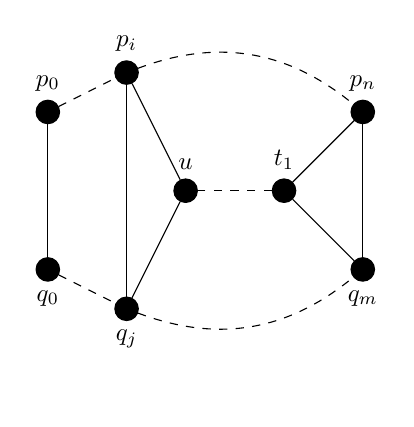
\begin{tikzpicture}[
		scale=1,
		every node/.style={circle, draw, minimum size=1mm, scale=0.9},
		every label/.append style={rectangle}
	]
  \node (p0) [label=above:$p_0$, fill] at (-2cm, 1cm) {};
  \node (pn) [label=above:$p_n$, fill] at (2cm, 1cm) {};
  \node (q0) [label=below:$q_0$, fill] at (-2cm, -1cm) {};
  \node (qn) [label=below:$q_m$, fill] at (2cm, -1cm) {};
  \node (t0) [label=above:$u$, fill] at (-0.25cm, 0cm) {};
  \node (t1) [label=above:$t_1$, fill] at (1cm, 0cm) {};
  \node (pi) [label=above:$p_i$, fill] at (-1cm, 1.5cm) {};
  \node (qj) [label=below:$q_j$, fill] at (-1cm, -1.5cm) {};
  \node (null) [draw=none] at (270:2.5cm) {};
  \draw (p0) edge (pi) [dashed];
  \draw (pi) edge [bend left] (pn) [dashed];
  \draw (q0) edge (qj) [dashed];
  \draw (qj) edge [bend right] (qn) [dashed];
  \draw (p0) edge (q0);
  \draw (pn) edge (qn);
  \draw (pi) edge (qj);
  \draw (pn) edge (t1);
  \draw (qn) edge (t1);
  \draw (t1) edge (t0) [dashed];
  \draw (pi) edge (t0);
  \draw (qj) edge (t0);
\end{tikzpicture}
$\qquad$
\begin{tikzpicture}[
		scale=1,
		every node/.style={circle, draw, minimum size=1mm, scale=0.9},
		every label/.append style={rectangle}
	]
  \node (null) [draw=none] at (0cm, 0cm) {$\rightarrow$};
  \node (null) [draw=none] at (270:2.5cm) {};
\end{tikzpicture}
$\qquad$
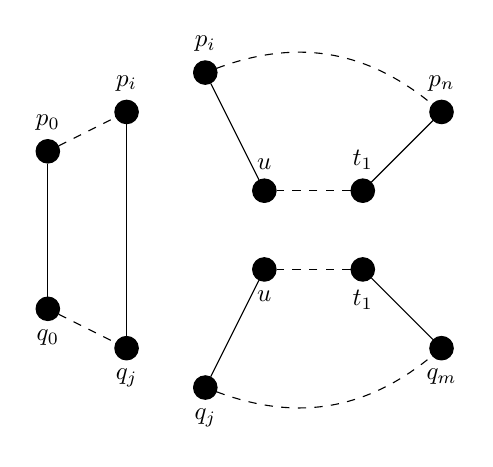
\begin{tikzpicture}[
		scale=1,
		every node/.style={circle, draw, minimum size=1mm, scale=0.9},
		every label/.append style={rectangle}
	]
  \node (p0) [label=above:$p_0$, fill] at (-3cm, 1cm) {};
  \node (q0) [label=below:$q_0$, fill] at (-3cm, -1cm) {};
  \node (pi) [label=above:$p_i$, fill] at (-2cm, 1.5cm) {};
  \node (qj) [label=below:$q_j$, fill] at (-2cm, -1.5cm) {};
  
  \node (pi_1) [label=above:$p_i$, fill] at (-1cm, 2cm) {};
  \node (pn) [label=above:$p_n$, fill] at (2cm, 1.5cm) {};
  \node (t0) [label=above:$u$, fill] at (-0.25cm, 0.5cm) {};
  \node (t1) [label=above:$t_1$, fill] at (1cm, 0.5cm) {};
  
  \node (qj_1) [label=below:$q_j$, fill] at (-1cm, -2cm) {};
  \node (qn) [label=below:$q_m$, fill] at (2cm, -1.5cm) {};
  \node (t0_1) [label=below:$u$, fill] at (-0.25cm, -0.5cm) {};
  \node (t1_1) [label=below:$t_1$, fill] at (1cm, -0.5cm) {};
  \node (null) [draw=none] at (270:2.5cm) {};
  \draw (p0) edge (pi) [dashed];
  \draw (pi_1) edge [bend left] (pn) [dashed];
  \draw (q0) edge (qj) [dashed];
  \draw (qj_1) edge [bend right] (qn) [dashed];
  \draw (p0) edge (q0);
  \draw (pi) edge (qj);
  \draw (pn) edge (t1);
  \draw (qn) edge (t1_1);
  \draw (t1) edge (t0) [dashed];
  \draw (t1_1) edge (t0_1) [dashed];
  \draw (pi_1) edge (t0);
  \draw (qj_1) edge (t0_1);
\end{tikzpicture}
\hfill\\
\textbf{Figure 2.2} The case $p_i\ne p_0$ or $q_i\ne q_0$.
\end{center}

\noindent To color the remaining graph we recurse on both the region
bounded by the $p_ip_n$-path and $ut_1$-path, and the region bounded by the $ut_1$-path and $q_jp_m$-path.
If $p_i=p_0$ and $q_j=q_0$ we are done and this mimicks the case of a $t_0t_1$ path in with $u=t_0$.
If $p_i\ne p_0$ or $q_j\ne q_0$ we handle the remaining subgraph by recursing on the region bounded by the
$p_0p_i$-path and $q_0p_j$-path. Note each recursive step is independant and vertex marks are shared,
thus the algorithm may instead proceed iteratively by pushing paths, represented by their start and end
vertices, into a stack or queue.

\subsection*{Time Complexity}

\noindent Locating $t_1$ requires a single neighbor lookup. The amortized complexity of a neighbor lookup is
$O(|E|/|V|)$. Each vertex may be $t_1$ at most once so over the entire graph we perform at most $|V|$ neighbor
lookups. In planar graphs $|E|\le 3|V|-6$, and $O(|E|)=O(|V|)$. Therefore, the
amortized complexity of this step is $O(|V|^2/|V|)=O(|V|)$. We also perform at most one breadth first
search from each $t_1$ with complexity $O(|V|)$. Therefore the complexity of the serach step over the
entire graph is $O(|V|^2)$. This gives us an overall amortized complexity of $O(|V|+|V|^2)=O(|V|^2)$.

\section{Path $3$-Choosing Plane Graphs}

The following is a restatment of a theorem of Hartman [r] and Skrekovski [s]. We provide a modification of
the proof that limits each inductive step to considering a single vertex and its set of neighbors. In this way
the proof follows a similar process to that of Thomassen [n] and yields a linear time implementation as suggested
by Hartman [r] detailed in following sections.\\

\noindent Suppose $C$ is
the outer cycle of a weakly triangulated plane graph $G$. Using notation from [r] for $u,v\in V(C)$ we
let $C[u,v]$ denote the path from $u$ to $v$ clockwise along the outer face. If we wish to exclude $u$ or $v$
from this path we will use parenthesis, $C(u,v)$. Similarly, for $v\in V(G)$ and
$u,w\in N(v)$ we let $[u,w]_v$ denote the path from $u$ to $w$ clockwise around $v$, assuming triangulated
faces.\\

\noindent Note that in all figures solid circles denote vertices yet to be colored, and colored vertices will
be labeled with their assigned color. We have $\alpha$ denote the current color and a label $\beta$ represent
coloring $v$ from $L(v)\setminus\{\alpha\}$. If a vertex $v$ is unlabled it represents arbitrary coloring from
$L(v)$.\\

\begin{adjustwidth}{1.5em}{1.5em}
\noindent\textbf{Theorem 2.} Let $G$ be a $2$-connected weakly triangulated plane graph, or a complete graph
on one or two vertics, with outer face $C$. 
Let $x,y\in V(C)$ be not necessarily distinct, potentially precolored vertices. Let $p\in C[x,y]$ be precolored some
color $\alpha$. Suppose $L(v)$ assigns a list of colors to each $v\in V(G)$ that has not been precolored such that
\[
    \begin{array}{ll}
	    |L(v)|\ge 1 & \text{if } v=x \text{ or } v=y;\\
	    |L(v)|\ge 2 & \text{if } v\in V(C)\setminus\{x,y\};\\
	    |L(v)|\ge 3 & \text{otherwise.}
    \end{array}
\]
If $p\ne x$, let $\alpha\not\in L(v)$ for
any $v\in V(C[x,p))$. Also assume the precoloring is a path coloring.\\

\noindent The coloring may be extended to
a path choosing of $G$ from $L$ such that $x$, $y$, and $p$ each recieve at most one same color neighbor. If
$x=y$ then $x$ and $y$ recieve no same color neighbors. If $y=p$, or $y$ is immediately prior to
$p$ on the outer face and $\alpha\not\in L(y)$, then $y$ recieves no same color neighbors.\\
\end{adjustwidth}

\begin{proof}
If $|V(G)\le 3$ the theorem easily follows. Suppose $|V(G)|>3$ and the theorem
holds for all graphs $H$ with $|V(H)|<|V(G)|$. Let
$C=c_0c_1\ldots c_n$ denote, in clockwise order, the outer face of $G$ with $p=c_0$.
There are several cases to consider. Let $c_i$ be the next vertex in $V(C)\cap N(p)$ counterclockwise from $c_n$.
Let $G_0$ be the subgraph bounded by the cycle formed from $C[c_i,c_n]$ and $[c_n,c_i]_p$. If $c_i\ne c_1$ let
$G_1$ be the sugbraph bounded by the cycle formed from $C[p,c_i]$ and the edge $pc_i$. As seen in Figure
3.1 $G=G_0\cup G_1$ and $V(G_0)\cap V(G_1)=\{c_i\}$.
We will display in each case that the inductive hypothesis holds for each subgraph and their union still
forms a path choosing of $G$ from $L$.
If $c_i=c_1$ we will say $G_1$ does not exist and handle this case specially noting $G_0=G-p$.

\begin{center}
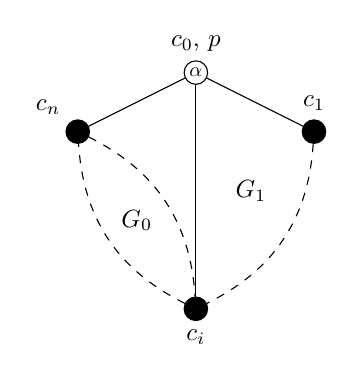
\begin{tikzpicture}[
		scale=1,
		every node/.style={circle, draw, minimum size=1mm, scale=0.9},
		every label/.append style={rectangle}
	]
  \node (c_n) [label=above left:$c_n$, fill] at (-1.5cm, 1.25cm) {};
  \node (p) [label=above:{$c_0$, $p$}] at (0cm, 2cm) {};
  \node (p_label) [draw=none, scale=0.8] at (0cm, 2cm) {$\alpha$};
  \node (c_1) [label=above:$c_1$, fill] at (1.5cm, 1.25cm) {};
  \node (c_i) [label=below:$c_i$, fill] at (0cm, -1cm) {};
  \node (G_0) [draw=none, ] at (-0.75cm, 0.12cm) {$G_0$};
  \node (G_1) [draw=none] at (0.7cm, 0.5cm) {$G_1$};
  \node (null) [draw=none] at (270:1.5cm) {};
  \draw (c_i) edge [bend left] (c_n) [dashed];
  \draw (c_n) edge [bend left] (c_i) [dashed];
  \draw (c_n) edge (p);
  \draw (p) edge (c_1);
  \draw (p) edge (c_i);
  \draw (c_1) edge [bend left] (c_i) [dashed];
\end{tikzpicture}
\hfill\\
\textbf{Figure 3.1} The subdivision of $G$ into $G_0$ and $G_1$.
\end{center}

\noindent For all $v\in (N(p)\cap V(G_0))\setminus\{x,y\}$ we note if $v=c_n$ or $v=c_i$
then $|L(v)|\ge 2$, and $|L(v)|\ge3$ otherwise. We define a new list assignment $L_0$
such that $L_0(v)=L(v)\setminus\{\alpha\}$ for
$v\in N(p)\cap V(G_0)$, and $L_0(v)=L(v)$ for $v\in V(G_0)\setminus N(p)$. Note that all
$v\in N(p)\cap V(G_0)$ will be on the outer face of $G_0$. Thus $|L_0(v)|\ge 3$ for all interior
vertices $v$ of $G_0$. Except for a few special cases for $y$ mentioned below, $|L_0(v)|\ge 1$ for all
$v\in\{x,y,c_i,c_n\}$. Finally, $|L_0(v)|\ge2$ for all other $v$ on the outer face of $G_0$. By choosing $G_0$ from
$L_0$ we ensure either $p$ recieves no new $\alpha$ colored neighbors in $G_0$. If $c_i$ is colored $\alpha$
then $p$ recieves no $\alpha$ colored neighbors in $G_1$ other than $c_i$.\\

\noindent If $\alpha\in L(y)$ and $y\in V(G_0)\cap N(p)$ it may be that $|L_0(y)|=0$. To handle this we
first note $y\in\{c_n, c_i\}$. The case $y=c_i$ will require no special treatment as $c_i$ will
naturally be colored $\alpha$. Suppose $\alpha\in L(y)$ and $y=c_n$. Then $x=p$ as otherwise $y\in C[x,p)$ and
$\alpha\not\in L(y)$. Color $y$ with $\alpha$ and apply the inductive hypothesis to choose
$G$ from $L$ with $x'=y$, $y'=x$, and $p'=y$. Otherwise suppose if $\alpha\in L(y)$ then $y\ne c_n$.

\begin{center}
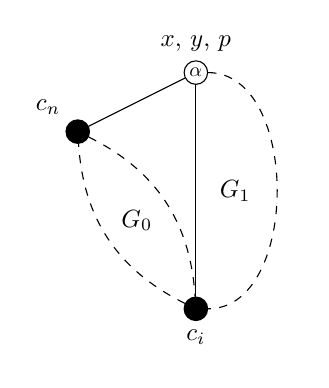
\begin{tikzpicture}[
		scale=1,
		every node/.style={circle, draw, minimum size=1mm, scale=0.9},
		every label/.append style={rectangle}
	]
  \node (c_n) [label=above left:$c_n$, fill] at (-1.5cm, 1.25cm) {};
  \node (p) [label=above:{$x$, $y$, $p$}] at (0cm, 2cm) {};
  \node (p_label) [draw=none, scale=0.8] at (0cm, 2cm) {$\alpha$};
  \node (c_i) [label=below:$c_i$, fill] at (0cm, -1cm) {};
  \node (G_0) [draw=none, ] at (-0.75cm, 0.12cm) {$G_0$};
  \node (G_1) [draw=none] at (0.5cm, 0.5cm) {$G_1$};
  \node (null) [draw=none] at (270:1.5cm) {};
  \draw (c_i) edge [bend left] (c_n) [dashed];
  \draw (c_n) edge [bend left] (c_i) [dashed];
  \draw (c_n) edge (p);
  \draw (p) edge (c_i);
  \draw (p) edge [bend left=90] (c_i) [dashed];
\end{tikzpicture}
$\quad$
\begin{tikzpicture}[
		scale=1,
		every node/.style={circle, draw, minimum size=1mm, scale=0.9},
		every label/.append style={rectangle}
	]
  \node (null) [draw=none] at (0cm, 0.5cm) {$\rightarrow$};
  \node (null) [draw=none] at (270:1.5cm) {};
\end{tikzpicture}
$\quad$
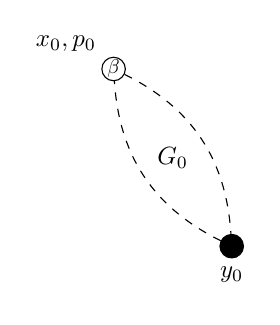
\begin{tikzpicture}[
		scale=1,
		every node/.style={circle, draw, minimum size=1mm, scale=0.9},
		every label/.append style={rectangle}
	]
  \node (c_n) [label=above left:{$x_0,p_0$}] at (-1.5cm, 1.25cm) {};
  \node (c_i) [label=below:$y_0$, fill] at (0cm, -1cm) {};
  \node (c_n_label) [draw=none, scale=0.8] at (-1.5cm, 1.25cm) {$\beta$};
  \node (G_0) [draw=none] at (-0.75cm, 0.12cm) {$G_0$};
  \node (null) [draw=none] at (270:1.5cm) {};
  \draw (c_i) edge [bend left] (c_n) [dashed];
  \draw (c_n) edge [bend left] (c_i) [dashed];
\end{tikzpicture}
$\quad$
\begin{tikzpicture}[
		scale=1,
		every node/.style={circle, draw, minimum size=1mm, scale=0.9},
		every label/.append style={rectangle}
	]
  \node (null) [draw=none] at (0cm, 0.5cm) {$\rightarrow$};
  \node (null) [draw=none] at (270:1.5cm) {};
\end{tikzpicture}
$\quad$
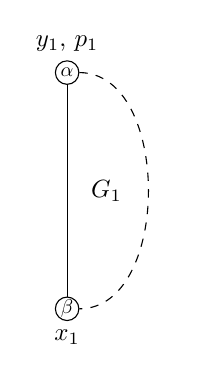
\begin{tikzpicture}[
		scale=1,
		every node/.style={circle, draw, minimum size=1mm, scale=0.9},
		every label/.append style={rectangle}
	]
  \node (p) [label=above:{$y_1$, $p_1$}] at (0cm, 2cm) {};
  \node (p_label) [draw=none, scale=0.8] at (0cm, 2cm) {$\alpha$};
  \node (c_i) [label=below:$x_1$] at (0cm, -1cm) {};
  \node (c_i_label) [draw=none, scale=0.8] at (0cm, -1cm) {$\beta$};
  \node (G_1) [draw=none] at (0.5cm, 0.5cm) {$G_1$};
  \node (null) [draw=none] at (270:1.5cm) {};
  \draw (p) edge (c_i);
  \draw (p) edge [bend left=90] (c_i) [dashed];
\end{tikzpicture}
\hfill\\
\textbf{Figure 3.2} The case $x=y=p$.
\end{center}

\noindent Suppose $x=y=p$. Color $c_i$ from $L_0(c_i)$. Apply the inductive hypothesis to choose $G_0$ from
$L$ with $x_0=c_n$, $y_0=p_0=c_i$. If $G_1$ exists we apply the inductive hypothesis again to choose $G_1$ from
$L$ with $x_1=c_i$, $y_1=y$, and $p_1=p$. Since $c_i$ recieves at most one neighbor in each $G_0$ and $G_1$, the
combined coloring forms a path choosing of $G$ from $L$.

\begin{center}
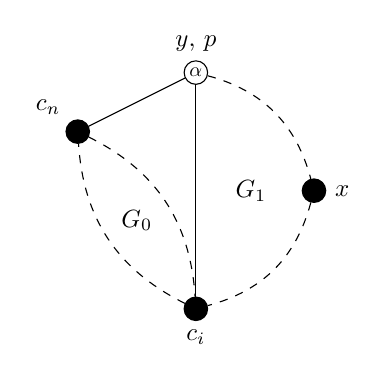
\begin{tikzpicture}[
		scale=1,
		every node/.style={circle, draw, minimum size=1mm, scale=0.9},
		every label/.append style={rectangle}
	]
  \node (c_n) [label=above left:$c_n$, fill] at (-1.5cm, 1.25cm) {};
  \node (p) [label=above:{$y$, $p$}] at (0cm, 2cm) {};
  \node (p_label) [draw=none, scale=0.8] at (0cm, 2cm) {$\alpha$};
  \node (x) [label=right:$x$, fill] at (1.5cm, 0.5cm) {};
  \node (c_i) [label=below:$c_i$, fill] at (0cm, -1cm) {};
  \node (G_0) [draw=none, ] at (-0.75cm, 0.12cm) {$G_0$};
  \node (G_1) [draw=none] at (0.7cm, 0.5cm) {$G_1$};
  \node (null) [draw=none] at (270:1.5cm) {};
  \draw (c_i) edge [bend left] (c_n) [dashed];
  \draw (c_n) edge [bend left] (c_i) [dashed];
  \draw (c_n) edge (p);
  \draw (p) edge (c_i);
  \draw (p) edge [bend left] (x) [dashed];
  \draw (x) edge [bend left] (c_i) [dashed];
\end{tikzpicture}
$\quad$
\begin{tikzpicture}[
		scale=1,
		every node/.style={circle, draw, minimum size=1mm, scale=0.9},
		every label/.append style={rectangle}
	]
  \node (null) [draw=none] at (0cm, 0.5cm) {$\rightarrow$};
  \node (null) [draw=none] at (270:1.5cm) {};
\end{tikzpicture}
$\quad$
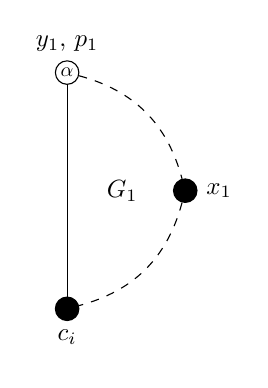
\begin{tikzpicture}[
		scale=1,
		every node/.style={circle, draw, minimum size=1mm, scale=0.9},
		every label/.append style={rectangle}
	]
  \node (p) [label=above:{$y_1$, $p_1$}] at (0cm, 2cm) {};
  \node (p_label) [draw=none, scale=0.8] at (0cm, 2cm) {$\alpha$};
  \node (x) [label=right:$x_1$, fill] at (1.5cm, 0.5cm) {};
  \node (c_i) [label=below:$c_i$,fill] at (0cm, -1cm) {};
  \node (G_1) [draw=none] at (0.7cm, 0.5cm) {$G_1$};
  \node (null) [draw=none] at (270:1.5cm) {};
  \draw (p) edge (c_i);
  \draw (p) edge [bend left] (x) [dashed];
  \draw (x) edge [bend left] (c_i) [dashed];
\end{tikzpicture}
$\quad$
\begin{tikzpicture}[
		scale=1,
		every node/.style={circle, draw, minimum size=1mm, scale=0.9},
		every label/.append style={rectangle}
	]
  \node (null) [draw=none] at (0cm, 0.5cm) {$\rightarrow$};
  \node (null) [draw=none] at (270:1.5cm) {};
\end{tikzpicture}
$\quad$
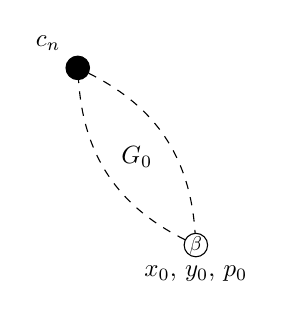
\begin{tikzpicture}[
		scale=1,
		every node/.style={circle, draw, minimum size=1mm, scale=0.9},
		every label/.append style={rectangle}
	]
  \node (c_n) [label=above left:{$c_n$}, fill] at (-1.5cm, 1.25cm) {};
  \node (c_i) [label=below:{$x_0$, $y_0$, $p_0$}] at (0cm, -1cm) {};
  \node (c_i_label) [draw=none, scale=0.8] at (0cm, -1cm) {$\beta$};
  \node (G_0) [draw=none] at (-0.75cm, 0.12cm) {$G_0$};
  \node (null) [draw=none] at (270:1.5cm) {};
  \draw (c_i) edge [bend left] (c_n) [dashed];
  \draw (c_n) edge [bend left] (c_i) [dashed];
\end{tikzpicture}
\hfill\\
\textbf{Figure 3.3} The case $y=p$, $x\ne p$, and $c_i\in C[x,p)$ (shown is the case $x\ne c_i$).
\end{center}

\noindent Suppose $y=p$, $x\ne p$, and $c_i\in C[x,p)$. If $G_1$ exists, apply
the inductive hypothesis to choose $G_1$ from $L$ with $x_1=x$, $y_1=y$, and $p_1=p$.
Apply the inductive hypothesis to choose $G_0$ from
$L_0$ with $x_0=y_0=p_0=c_i$. If $G_1$ exists note $c_i$ was precolored from the choosing of $G_1$ and recieves
no same color neighbors in $G_0$. Thus the combined coloring forms a path choosing of $G$ from $L$.

\begin{center}
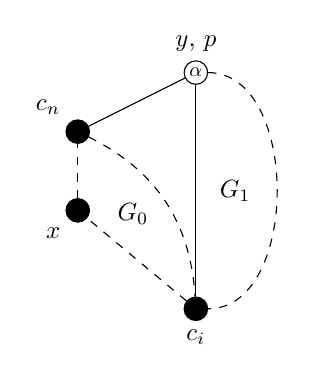
\begin{tikzpicture}[
		scale=1,
		every node/.style={circle, draw, minimum size=1mm, scale=0.9},
		every label/.append style={rectangle}
	]
  \node (c_n) [label=above left:$c_n$, fill] at (-1.5cm, 1.25cm) {};
  \node (p) [label=above:{$y$, $p$}] at (0cm, 2cm) {};
  \node (p_label) [draw=none, scale=0.8] at (0cm, 2cm) {$\alpha$};
  \node (x) [label=below left:$x$, fill] at (-1.5cm, 0.25cm) {};
  \node (c_i) [label=below:$c_i$, fill] at (0cm, -1cm) {};
  \node (G_0) [draw=none, ] at (-0.8cm, 0.2cm) {$G_0$};
  \node (G_1) [draw=none] at (0.5cm, 0.5cm) {$G_1$};
  \node (null) [draw=none] at (270:1.5cm) {};
  \draw (c_i) edge (x) [dashed];
  \draw (x) edge (c_n) [dashed];
  \draw (c_n) edge [bend left] (c_i) [dashed];
  \draw (c_n) edge (p);
  \draw (p) edge (c_i);
  \draw (p) edge [bend left=90] (c_i) [dashed];
\end{tikzpicture}
$\quad$
\begin{tikzpicture}[
		scale=1,
		every node/.style={circle, draw, minimum size=1mm, scale=0.9},
		every label/.append style={rectangle}
	]
  \node (null) [draw=none] at (0cm, 0.5cm) {$\rightarrow$};
  \node (null) [draw=none] at (270:1.5cm) {};
\end{tikzpicture}
$\quad$
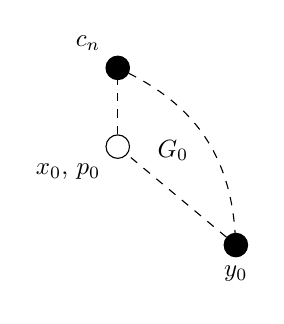
\begin{tikzpicture}[
		scale=1,
		every node/.style={circle, draw, minimum size=1mm, scale=0.9},
		every label/.append style={rectangle}
	]
  \node (c_n) [label=above left:$c_n$, fill] at (-1.5cm, 1.25cm) {};
  \node (x) [label=below left:{$x_0$, $p_0$}] at (-1.5cm, 0.25cm) {};
  \node (c_i) [label=below:$y_0$, fill] at (0cm, -1cm) {};
  \node (G_0) [draw=none, ] at (-0.8cm, 0.2cm) {$G_0$};
  \node (null) [draw=none] at (270:1.5cm) {};
  \draw (c_i) edge (x) [dashed];
  \draw (x) edge (c_n) [dashed];
  \draw (c_n) edge [bend left] (c_i) [dashed];
\end{tikzpicture}
$\quad$
\begin{tikzpicture}[
		scale=1,
		every node/.style={circle, draw, minimum size=1mm, scale=0.9},
		every label/.append style={rectangle}
	]
  \node (null) [draw=none] at (0cm, 0.5cm) {$\rightarrow$};
  \node (null) [draw=none] at (270:1.5cm) {};
\end{tikzpicture}
$\quad$
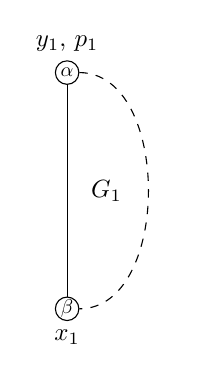
\begin{tikzpicture}[
		scale=1,
		every node/.style={circle, draw, minimum size=1mm, scale=0.9},
		every label/.append style={rectangle}
	]
  \node (p) [label=above:{$y_1$, $p_1$}] at (0cm, 2cm) {};
  \node (p_label) [draw=none, scale=0.8] at (0cm, 2cm) {$\alpha$};
  \node (c_i) [label=below:$x_1$] at (0cm, -1cm) {};
  \node (c_i_label) [draw=none, scale=0.8] at (0cm, -1cm) {$\beta$};
  \node (G_1) [draw=none] at (0.5cm, 0.5cm) {$G_1$};
  \node (null) [draw=none] at (270:1.5cm) {};
  \draw (p) edge (c_i);
  \draw (p) edge [bend left=90] (c_i) [dashed];
\end{tikzpicture}
\hfill\\
\textbf{Figure 3.4} The case $y=p$, $x\ne p$, and $c_i\not\in C[x,p)$.
\end{center}

\noindent Suppose $y=p$, $x\ne p$, and $c_i\not\in C[x,p)$. Color $x$ from $L_0(x)$ and apply the inductive
hypothesis to choose
$G_0$ from $L_0$ with $x_0=p_0=x$ and $y_0=c_i$. If $G_1$ exists we apply the inductive hypothesis again to
choose $G_1$ from $L$ with $x_1=c_i$, $y_1=y$, and $p_1=p$. Notice $c_i$ recieves at most one same color
neighbor in each $G_0$ and $G_1$. 

\begin{center}
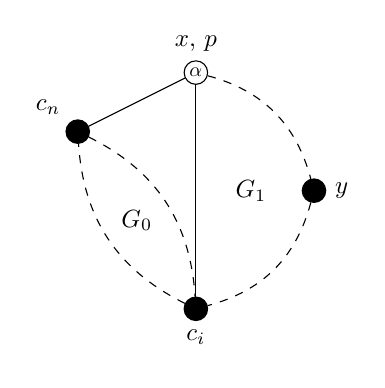
\begin{tikzpicture}[
		scale=1,
		every node/.style={circle, draw, minimum size=1mm, scale=0.9},
		every label/.append style={rectangle}
	]
  \node (c_n) [label=above left:$c_n$, fill] at (-1.5cm, 1.25cm) {};
  \node (p) [label=above:{$x$, $p$}] at (0cm, 2cm) {};
  \node (p_label) [draw=none, scale=0.8] at (0cm, 2cm) {$\alpha$};
  \node (y) [label=right:$y$, fill] at (1.5cm, 0.5cm) {};
  \node (c_i) [label=below:$c_i$, fill] at (0cm, -1cm) {};
  \node (G_0) [draw=none, ] at (-0.75cm, 0.12cm) {$G_0$};
  \node (G_1) [draw=none] at (0.7cm, 0.5cm) {$G_1$};
  \node (null) [draw=none] at (270:1.5cm) {};
  \draw (c_i) edge [bend left] (c_n) [dashed];
  \draw (c_n) edge [bend left] (c_i) [dashed];
  \draw (c_n) edge (p);
  \draw (p) edge (c_i);
  \draw (p) edge [bend left] (y) [dashed];
  \draw (y) edge [bend left] (c_i) [dashed];
\end{tikzpicture}
$\quad$
\begin{tikzpicture}[
		scale=1,
		every node/.style={circle, draw, minimum size=1mm, scale=0.9},
		every label/.append style={rectangle}
	]
  \node (null) [draw=none] at (0cm, 0.5cm) {$\rightarrow$};
  \node (null) [draw=none] at (270:1.5cm) {};
\end{tikzpicture}
$\quad$
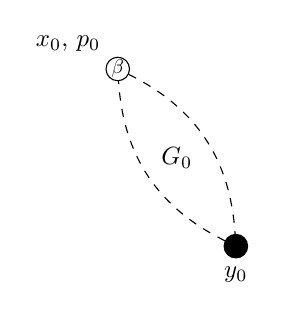
\begin{tikzpicture}[
		scale=1,
		every node/.style={circle, draw, minimum size=1mm, scale=0.9},
		every label/.append style={rectangle}
	]
  \node (c_n) [label=above left:{$x_0$, $p_0$}] at (-1.5cm, 1.25cm) {};
  \node (c_n_label) [draw=none, scale=0.8] at (-1.5cm, 1.25cm) {$\beta$};
  \node (c_i) [label=below:{$y_0$}, fill] at (0cm, -1cm) {};
  \node (G_0) [draw=none] at (-0.75cm, 0.12cm) {$G_0$};
  \node (null) [draw=none] at (270:1.5cm) {};
  \draw (c_i) edge [bend left] (c_n) [dashed];
  \draw (c_n) edge [bend left] (c_i) [dashed];
\end{tikzpicture}
$\quad$
\begin{tikzpicture}[
		scale=1,
		every node/.style={circle, draw, minimum size=1mm, scale=0.9},
		every label/.append style={rectangle}
	]
  \node (null) [draw=none] at (0cm, 0.5cm) {$\rightarrow$};
  \node (null) [draw=none] at (270:1.5cm) {};
\end{tikzpicture}
$\quad$
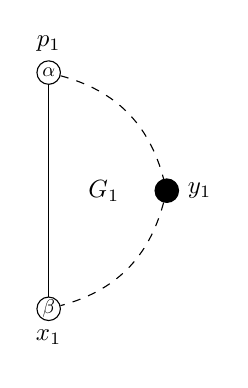
\begin{tikzpicture}[
		scale=1,
		every node/.style={circle, draw, minimum size=1mm, scale=0.9},
		every label/.append style={rectangle}
	]
  \node (p) [label=above:$p_1$] at (0cm, 2cm) {};
  \node (p_label) [draw=none, scale=0.8] at (0cm, 2cm) {$\alpha$};
  \node (y) [label=right:$y_1$, fill] at (1.5cm, 0.5cm) {};
  \node (c_i) [label=below:$x_1$] at (0cm, -1cm) {};
  \node (c_i_label) [draw=none, scale=0.8] at (0cm, -1cm) {$\beta$};
  \node (G_1) [draw=none] at (0.7cm, 0.5cm) {$G_1$};
  \node (null) [draw=none] at (270:1.5cm) {};
  \draw (p) edge (c_i);
  \draw (p) edge [bend left] (y) [dashed];
  \draw (y) edge [bend left] (c_i) [dashed];
\end{tikzpicture}
\hfill\\
\textbf{Figure 3.5} The case $x=p$, $y\ne p$, and $c_i\in C(y,x)$.
\end{center}

\noindent Suppose $x=p$, $y\ne p$, and $c_i\in C(y,x)$. Apply the
inductive hypothesis to choose $G_0$ from $L_0$ with $x_0=p_0=c_n$ and $y_0=c_i$. In this case $G_1$ must exist
and we apply the inductive
hypothesis to choose $G_1$ from $L$ with $x_1=c_i$, $y_1=y$, and $p_1=p$. Notice $c_i$ recieves at most one same
color neighbor in each $G_0$ and $G_1$.

\begin{center}
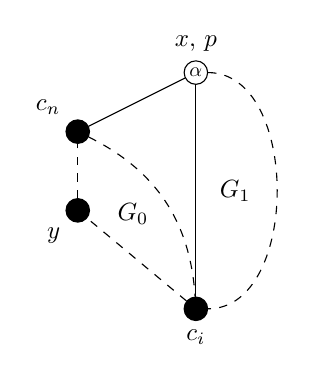
\begin{tikzpicture}[
		scale=1,
		every node/.style={circle, draw, minimum size=1mm, scale=0.9},
		every label/.append style={rectangle}
	]
  \node (c_n) [label=above left:$c_n$, fill] at (-1.5cm, 1.25cm) {};
  \node (p) [label=above:{$x$, $p$}] at (0cm, 2cm) {};
  \node (p_label) [draw=none, scale=0.8] at (0cm, 2cm) {$\alpha$};
  \node (y) [label=below left:$y$, fill] at (-1.5cm, 0.25cm) {};
  \node (c_i) [label=below:$c_i$, fill] at (0cm, -1cm) {};
  \node (G_0) [draw=none, ] at (-0.8cm, 0.2cm) {$G_0$};
  \node (G_1) [draw=none] at (0.5cm, 0.5cm) {$G_1$};
  \node (null) [draw=none] at (270:1.5cm) {};
  \draw (c_i) edge (y) [dashed];
  \draw (y) edge (c_n) [dashed];
  \draw (c_n) edge [bend left] (c_i) [dashed];
  \draw (c_n) edge (p);
  \draw (p) edge (c_i);
  \draw (p) edge [bend left=90] (c_i) [dashed];
\end{tikzpicture}
$\quad$
\begin{tikzpicture}[
		scale=1,
		every node/.style={circle, draw, minimum size=1mm, scale=0.9},
		every label/.append style={rectangle}
	]
  \node (null) [draw=none] at (0cm, 0.5cm) {$\rightarrow$};
  \node (null) [draw=none] at (270:1.5cm) {};
\end{tikzpicture}
$\quad$
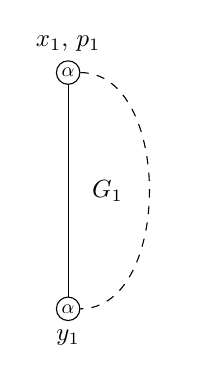
\begin{tikzpicture}[
		scale=1,
		every node/.style={circle, draw, minimum size=1mm, scale=0.9},
		every label/.append style={rectangle}
	]
  \node (p) [label=above:{$x_1$, $p_1$}] at (0cm, 2cm) {};
  \node (p_label) [draw=none, scale=0.8] at (0cm, 2cm) {$\alpha$};
  \node (c_i) [label=below:$y_1$] at (0cm, -1cm) {};
  \node (c_i_label) [draw=none, scale=0.8] at (0cm, -1cm) {$\alpha$};
  \node (G_1) [draw=none] at (0.5cm, 0.5cm) {$G_1$};
  \node (null) [draw=none] at (270:1.5cm) {};
  \draw (p) edge (c_i);
  \draw (p) edge [bend left=90] (c_i) [dashed];
\end{tikzpicture}
$\quad$
\begin{tikzpicture}[
		scale=1,
		every node/.style={circle, draw, minimum size=1mm, scale=0.9},
		every label/.append style={rectangle}
	]
  \node (null) [draw=none] at (0cm, 0.5cm) {$\rightarrow$};
  \node (null) [draw=none] at (270:1.5cm) {};
\end{tikzpicture}
$\quad$
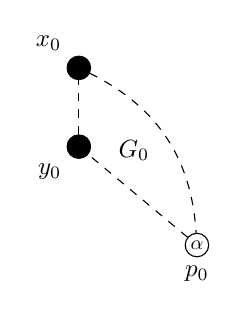
\begin{tikzpicture}[
		scale=1,
		every node/.style={circle, draw, minimum size=1mm, scale=0.9},
		every label/.append style={rectangle}
	]
  \node (c_n) [label=above left:$x_0$, fill] at (-1.5cm, 1.25cm) {};
  \node (y) [label=below left:$y_0$, fill] at (-1.5cm, 0.25cm) {};
  \node (c_i) [label=below:$p_0$] at (0cm, -1cm) {};
  \node (c_i_label) [draw=none, scale=0.8] at (0cm, -1cm) {$\alpha$};
  \node (G_0) [draw=none, ] at (-0.8cm, 0.2cm) {$G_0$};
  \node (null) [draw=none] at (270:1.5cm) {};
  \draw (c_i) edge (y) [dashed];
  \draw (y) edge (c_n) [dashed];
  \draw (c_n) edge [bend left] (c_i) [dashed];
\end{tikzpicture}
\hfill\\
\textbf{Figure 3.6} The case $x=p$, $y\ne p$, and $c_i\not\in C(y,x)$ (shown is the case $y\ne c_i$ and
$\alpha\in L(c_i)$).
\end{center}

\noindent Suppose $x=p$, $y\ne p$, and $c_i\not\in C(y,x)$. If
$\alpha\in L(c_i)$ we set $p_0=c_i$ and color $c_i$ with $\alpha$. Otherwise, set $p_0=c_n$ and color it with
the first color in $L_0(c_n)$, note $|L_0(c_i)|\ge 2$ in this case. Apply the inductive hypothesis to
choose $G_0$ from $L_0$ with $x_0=c_n$, $y_0=y$, and $p_0$. If $G_1$ exists, apply the inductive
hypothesis to choose $G_1$ from $L$ with $x_1=p_1=p$ and $y_1=c_i$. Notice if $p_0=c_i$, $c_i$ recieves at most
one same color neighbor in $G_0$ and the single same color neighbor $p$ in $G_1$. Furthermore, $p$ will recieve no
same color neighbor in $G_1$ other than $c_i$. If $p_0\ne c_i$, then $y_1=c_i$ is immediatley prior to
$p_1=p$ and $\alpha\not\in L(c_i)$. Thus $c_i$ will recieve no same color neighbors in $G_1$.

\begin{center}
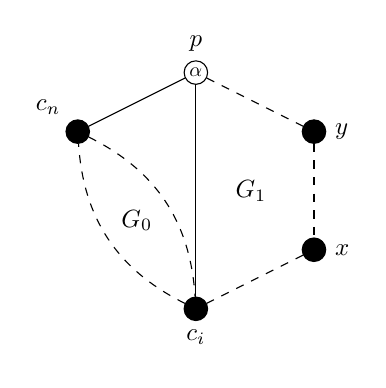
\begin{tikzpicture}[
		scale=1,
		every node/.style={circle, draw, minimum size=1mm, scale=0.9},
		every label/.append style={rectangle}
	]
  \node (c_n) [label=above left:$c_n$, fill] at (-1.5cm, 1.25cm) {};
  \node (p) [label=above:{$p$}] at (0cm, 2cm) {};
  \node (p_label) [draw=none, scale=0.8] at (0cm, 2cm) {$\alpha$};
  \node (y) [label=right:$y$, fill] at (1.5cm, 1.25cm) {};
  \node (x) [label=right:$x$, fill] at (1.5cm, -0.25cm) {};
  \node (c_i) [label=below:$c_i$, fill] at (0cm, -1cm) {};
  \node (G_0) [draw=none, ] at (-0.75cm, 0.12cm) {$G_0$};
  \node (G_1) [draw=none] at (0.7cm, 0.5cm) {$G_1$};
  \node (null) [draw=none] at (270:1.5cm) {};
  \draw (c_i) edge [bend left] (c_n) [dashed];
  \draw (c_n) edge [bend left] (c_i) [dashed];
  \draw (c_n) edge (p);
  \draw (p) edge (c_i);
  \draw (p) edge (y) [dashed];
  \draw (y) edge (x) [dashed];
  \draw (x) edge (c_i) [dashed];
\end{tikzpicture}
$\quad$
\begin{tikzpicture}[
		scale=1,
		every node/.style={circle, draw, minimum size=1mm, scale=0.9},
		every label/.append style={rectangle}
	]
  \node (null) [draw=none] at (0cm, 0.5cm) {$\rightarrow$};
  \node (null) [draw=none] at (270:1.5cm) {};
\end{tikzpicture}
$\quad$
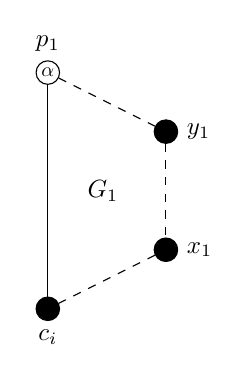
\begin{tikzpicture}[
		scale=1,
		every node/.style={circle, draw, minimum size=1mm, scale=0.9},
		every label/.append style={rectangle}
	]
  \node (p) [label=above:{$p_1$}] at (0cm, 2cm) {};
  \node (p_label) [draw=none, scale=0.8] at (0cm, 2cm) {$\alpha$};
  \node (y) [label=right:$y_1$, fill] at (1.5cm, 1.25cm) {};
  \node (x) [label=right:$x_1$, fill] at (1.5cm, -0.25cm) {};
  \node (c_i) [label=below:$c_i$, fill] at (0cm, -1cm) {};
  \node (G_1) [draw=none] at (0.7cm, 0.5cm) {$G_1$};
  \node (null) [draw=none] at (270:1.5cm) {};
  \draw (p) edge (c_i);
  \draw (p) edge (y) [dashed];
  \draw (y) edge (x) [dashed];
  \draw (x) edge (c_i) [dashed];
\end{tikzpicture}
$\quad$
\begin{tikzpicture}[
		scale=1,
		every node/.style={circle, draw, minimum size=1mm, scale=0.9},
		every label/.append style={rectangle}
	]
  \node (null) [draw=none] at (0cm, 0.5cm) {$\rightarrow$};
  \node (null) [draw=none] at (270:1.5cm) {};
\end{tikzpicture}
$\quad$
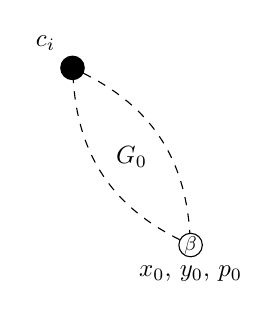
\begin{tikzpicture}[
		scale=1,
		every node/.style={circle, draw, minimum size=1mm, scale=0.9},
		every label/.append style={rectangle}
	]
  \node (c_n) [label=above left:$c_i$, fill] at (-1.5cm, 1.25cm) {};
  \node (c_i) [label=below:{$x_0$, $y_0$, $p_0$}] at (0cm, -1cm) {};
  \node (c_i_label) [draw=none, scale=0.8] at (0cm, -1cm) {$\beta$};
  \node (G_0) [draw=none, ] at (-0.75cm, 0.12cm) {$G_0$};
  \node (null) [draw=none] at (270:1.5cm) {};
  \draw (c_i) edge [bend left] (c_n) [dashed];
  \draw (c_n) edge [bend left] (c_i) [dashed];
\end{tikzpicture}
\hfill\\
\textbf{Figure 3.7} The case $x\ne p$, $y\ne p$, and $c_i\in C[x,p)$ (shown is the case $x\ne c_i$).
\end{center}

\noindent Suppose $x\ne p$, $y\ne p$, and $c_i\in C[x,p)$. In this case $G_1$ must exist and we apply
the inductive hypothesis to choose $G_1$ from $L$ with $x_1=x$, $y_1=y$, and $p_1=p$.
Apply the inductive hypothesis again to choose $G_0$ from
$L_0$ with $x_0=y_0=p_0=c_i$. Note that $c_i$ was precolored from the choosing of $G_1$ and recieves
no same color neighbors in $G_0$ so the combined coloring forms a path choosing of $G$ from $L$.

\begin{center}
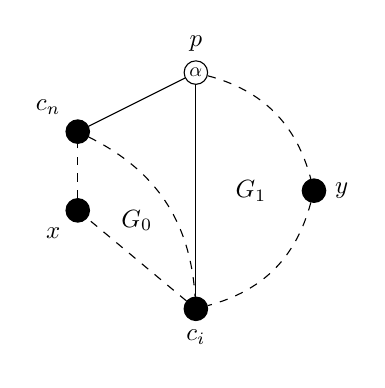
\begin{tikzpicture}[
		scale=1,
		every node/.style={circle, draw, minimum size=1mm, scale=0.9},
		every label/.append style={rectangle}
	]
  \node (c_n) [label=above left:$c_n$, fill] at (-1.5cm, 1.25cm) {};
  \node (p) [label=above:{$p$}] at (0cm, 2cm) {};
  \node (p_label) [draw=none, scale=0.8] at (0cm, 2cm) {$\alpha$};
  \node (x) [label=below left:$x$, fill] at (-1.5cm, 0.25cm) {};
  \node (y) [label=right:$y$, fill] at (1.5cm, 0.5cm) {};
  \node (c_i) [label=below:$c_i$, fill] at (0cm, -1cm) {};
  \node (G_0) [draw=none, ] at (-0.75cm, 0.12cm) {$G_0$};
  \node (G_1) [draw=none] at (0.7cm, 0.5cm) {$G_1$};
  \node (null) [draw=none] at (270:1.5cm) {};
  \draw (c_i) edge (x) [dashed];
  \draw (x) edge (c_n) [dashed];
  \draw (c_n) edge [bend left] (c_i) [dashed];
  \draw (c_n) edge (p);
  \draw (p) edge (c_i);
  \draw (p) edge [bend left] (y) [dashed];
  \draw (y) edge [bend left] (c_i) [dashed];
\end{tikzpicture}
$\quad$
\begin{tikzpicture}[
		scale=1,
		every node/.style={circle, draw, minimum size=1mm, scale=0.9},
		every label/.append style={rectangle}
	]
  \node (null) [draw=none] at (0cm, 0.5cm) {$\rightarrow$};
  \node (null) [draw=none] at (270:1.5cm) {};
\end{tikzpicture}
$\quad$
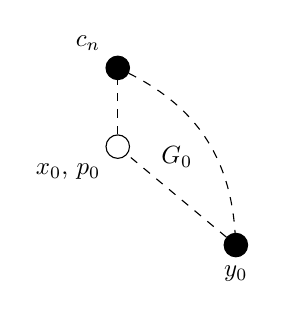
\begin{tikzpicture}[
		scale=1,
		every node/.style={circle, draw, minimum size=1mm, scale=0.9},
		every label/.append style={rectangle}
	]
  \node (c_n) [label=above left:{$c_n$}, fill] at (-1.5cm, 1.25cm) {};
  \node (x) [label=below left:{$x_0$, $p_0$}] at (-1.5cm, 0.25cm) {};
  \node (c_i) [label=below:{$y_0$}, fill] at (0cm, -1cm) {};
  \node (G_0) [draw=none] at (-0.75cm, 0.12cm) {$G_0$};
  \node (null) [draw=none] at (270:1.5cm) {};
  \draw (c_i) edge (x) [dashed];
  \draw (x) edge (c_n) [dashed];
  \draw (c_n) edge [bend left] (c_i) [dashed];
\end{tikzpicture}
$\quad$
\begin{tikzpicture}[
		scale=1,
		every node/.style={circle, draw, minimum size=1mm, scale=0.9},
		every label/.append style={rectangle}
	]
  \node (null) [draw=none] at (0cm, 0.5cm) {$\rightarrow$};
  \node (null) [draw=none] at (270:1.5cm) {};
\end{tikzpicture}
$\quad$
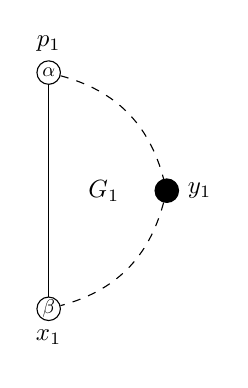
\begin{tikzpicture}[
		scale=1,
		every node/.style={circle, draw, minimum size=1mm, scale=0.9},
		every label/.append style={rectangle}
	]
  \node (p) [label=above:$p_1$] at (0cm, 2cm) {};
  \node (p_label) [draw=none, scale=0.8] at (0cm, 2cm) {$\alpha$};
  \node (y) [label=right:$y_1$, fill] at (1.5cm, 0.5cm) {};
  \node (c_i) [label=below:$x_1$] at (0cm, -1cm) {};
  \node (c_i_label) [draw=none, scale=0.8] at (0cm, -1cm) {$\beta$};
  \node (G_1) [draw=none] at (0.7cm, 0.5cm) {$G_1$};
  \node (null) [draw=none] at (270:1.5cm) {};
  \draw (p) edge (c_i);
  \draw (p) edge [bend left] (y) [dashed];
  \draw (y) edge [bend left] (c_i) [dashed];
\end{tikzpicture}
\hfill\\
\textbf{Figure 3.8} The case $x\ne p$, $y\ne p$, and $c_i\in C(y,x)$.
\end{center}

\noindent Suppose $x\ne p$, $y\ne p$, and $c_i\in C(y,x)$. Apply
the inductive hypothesis to choose $G_0$ from $L_0$ with $x_0=p_0=x$ and $y_0=c_i$. In this case $G_1$ must exist
and we apply the inductive
hypothesis again to choose $G_1$ from $L$ with $x_1=c_i$, $y_1=y$, and $p_1=p$. Notice $c_i$ recieves at most
one same color neighbor in each $G_0$ and $G_1$.

\begin{center}
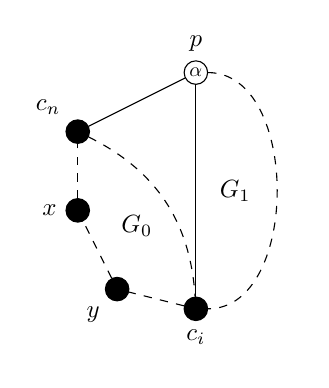
\begin{tikzpicture}[
		scale=1,
		every node/.style={circle, draw, minimum size=1mm, scale=0.9},
		every label/.append style={rectangle}
	]
  \node (c_n) [label=above left:$c_n$, fill] at (-1.5cm, 1.25cm) {};
  \node (p) [label=above:{$p$}] at (0cm, 2cm) {};
  \node (p_label) [draw=none, scale=0.8] at (0cm, 2cm) {$\alpha$};
  \node (x) [label=left:$x$, fill] at (-1.5cm, 0.25cm) {};
  \node (y) [label=below left:$y$, fill] at (-1cm, -0.75cm) {};
  \node (c_i) [label=below:$c_i$, fill] at (0cm, -1cm) {};
  \node (G_0) [draw=none, ] at (-0.75cm, 0.05cm) {$G_0$};
  \node (G_1) [draw=none] at (0.5cm, 0.5cm) {$G_1$};
  \node (null) [draw=none] at (270:1.5cm) {};
  \draw (c_i) edge (y) [dashed];
  \draw (y) edge (x) [dashed];
  \draw (x) edge (c_n) [dashed];
  \draw (c_n) edge [bend left] (c_i) [dashed];
  \draw (c_n) edge (p);
  \draw (p) edge (c_i);
  \draw (p) edge [bend left=90] (c_i) [dashed];
\end{tikzpicture}
$\quad$
\begin{tikzpicture}[
		scale=1,
		every node/.style={circle, draw, minimum size=1mm, scale=0.9},
		every label/.append style={rectangle}
	]
  \node (null) [draw=none] at (0cm, 0.5cm) {$\rightarrow$};
  \node (null) [draw=none] at (270:1.5cm) {};
\end{tikzpicture}
$\quad$
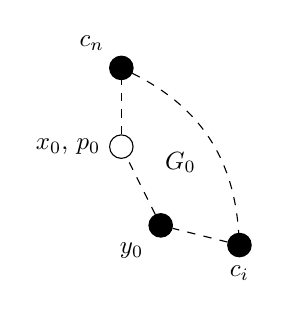
\begin{tikzpicture}[
		scale=1,
		every node/.style={circle, draw, minimum size=1mm, scale=0.9},
		every label/.append style={rectangle}
	]
  \node (c_n) [label=above left:{$c_n$}, fill] at (-1.5cm, 1.25cm) {};
  \node (x) [label=left:{$x_0$, $p_0$}] at (-1.5cm, 0.25cm) {};
  \node (y) [label=below left:$y_0$, fill] at (-1cm, -0.75cm) {};
  \node (c_i) [label=below:$c_i$, fill] at (0cm, -1cm) {};
  \node (G_0) [draw=none, ] at (-0.75cm, 0.05cm) {$G_0$};
  \node (null) [draw=none] at (270:1.5cm) {};
  \draw (c_i) edge (y) [dashed];
  \draw (y) edge (x) [dashed];
  \draw (x) edge (c_n) [dashed];
  \draw (c_n) edge [bend left] (c_i) [dashed];
\end{tikzpicture}
$\quad$
\begin{tikzpicture}[
		scale=1,
		every node/.style={circle, draw, minimum size=1mm, scale=0.9},
		every label/.append style={rectangle}
	]
  \node (null) [draw=none] at (0cm, 0.5cm) {$\rightarrow$};
  \node (null) [draw=none] at (270:1.5cm) {};
\end{tikzpicture}
$\quad$
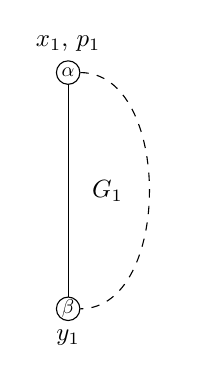
\begin{tikzpicture}[
		scale=1,
		every node/.style={circle, draw, minimum size=1mm, scale=0.9},
		every label/.append style={rectangle}
	]
  \node (p) [label=above:{$x_1$, $p_1$}] at (0cm, 2cm) {};
  \node (p_label) [draw=none, scale=0.8] at (0cm, 2cm) {$\alpha$};
  \node (c_i) [label=below:$y_1$] at (0cm, -1cm) {};
  \node (c_i_label) [draw=none, scale=0.8] at (0cm, -1cm) {$\beta$};
  \node (G_1) [draw=none] at (0.5cm, 0.5cm) {$G_1$};
  \node (null) [draw=none] at (270:1.5cm) {};
  \draw (p) edge (c_i);
  \draw (p) edge [bend left=90] (c_i) [dashed];
\end{tikzpicture}
\hfill\\
\textbf{Figure 3.9} The case $x\ne p$, $y\ne p$, and $c_i\in C(p,y]$ (shown is the case $y\ne c_i$ and
$\alpha\not\in L(c_i)$).
\end{center}

\noindent Finally, suppose $x\ne p$, $y\ne p$, and $c_i\in C(p,y]$. If
$\alpha\in L(c_i)$ we set $p_0=c_i$ and color $c_i$ with $\alpha$. Otherwise, define $p_0=c_1$ and color it from
$L_0(c_1)$, noting $|L_0(c_i)|\ge 2$ in this case. Apply the inductive hypothesis to
choose $G_0$ from $L_0$ with $x_0=x$, $y_0=y$, and $p_0$. If $G_1$ exists, apply the inductive again
hypothesis to choose $G_1$ from $L$ with $x_1=p_1=p$ and $y_1=c_i$. Note that $c_i$ was precolored by our
choosing of $G_0$. If $p_0=c_i$, $c_i$ recieves at most one same
color neighbor in $G_0$ and the single same color neighbor $p$ in $G_1$. Furthermore, $p$ will recieve no
same color neighbor in $G_1$ other than $c_i$. If $p_0\ne c_i$, then $y_1=c_i$ is immediatley prior to
$p_1=p$ and $\alpha\not\in L(c_i)$. Thus $c_i$ will recieve no same color neighbors in $G_1$.
\end{proof}

\subsection*{Implementing Hartman and Skrekovski's Algorithm}

Once again let the plane graph $G$ be represented as an incidence list and an ordering of edges around each
vertex following a planar embedding. Let the vertices $x$, $y$, and $p$ be provided. We will track subgraphs by
marking each vertex with a \emph{state} of \emph{interior},
\emph{face}, or \emph{colored}. Vertices will only change in state from \emph{interior} to \emph{face} to
\emph{colored}. We will also have a \emph{neighbor range} for all \emph{face} and \emph{colored} vertices
that will track the subset of the ordered incidence list included in the current outer face. To walk clockwise
along the outer face from some \emph{face} vertex we may simply proceed to the most counterclockwise neighbor in
its \emph{neighbor range}. To be able to perform the proceedure from the proof above
we must also determine where each \emph{face} vertex lies on the face in respect to $x$, $y$, and $p$. This
\emph{face location} property is nontrivial and is discussed in the following section.\\

\noindent Suppose the afformentioned properties tracked for each vertex. Note \emph{neighbor range}
for $p$ will begin at $c_i$ and proceed clockwise to $c_n$. We first check for the case $y=c_n$ and
$\alpha\in L(y)$ and perform the necessary coloring of $y$ and renaming of $x$, $y$, and $p$. Next proceed
counterclockwise through each $n\in N(p)$ starting with $c_n$. For each $n$ we perform the following:

\begin{enumerate}
\item if $n$ is interior, initialize its \emph{neighbor range} and set its \emph{state} to \emph{face};
\item contract the \emph{neighbor range} of $n$ to remove $p$ from its incidence list;
\item if $n\in C$ and $n\ne c_n$ terminate;
\item remove $\alpha$ from $L(n)$.
\end{enumerate}

\noindent Once the above procedure terminates we will have located $c_i$. The tracking of the subgraphs $G_0$ and $G_1$
are already almost complete by our tracking of \emph{state} and \emph{neighbor range}. It remains to determine
\emph{neighbor range} for $c_i$ in $G_0$ and $G_1$. This can be achieved by locating $p$ in $c_i$'s incidence list
and splitting the current \emph{neighbor range} of $c_i$ in two at the given edge. Comparing $c_i$, $x$, $y$, and
$p$, along with the \emph{face location} and \emph{state} properties for each we may determine which case to
apply and make the appropriate recursive calls on $G_0$ and $G_1$.

\subsection*{Efficient Tracking of Outer Face Location}


\begin{comment}
\begin{algorithm}
\LinesNumbered
\DontPrintSemicolon
\KwIn{Plane graph $G$ and paths $P=p_0\ldots p_n$ and $Q=q_0\ldots q_m$}
\Begin{
	\Repeat{$t_0\not\in P\cup Q$} {
		$t_0\longleftarrow$ vertex forming face with $p_0$ and $q_0$\;
		\If{$t_0 = p_1$} {
			$P\longleftarrow P - p_0$\;
		}
		\ElseIf{$t_0 = q_1$} {
			$Q\longleftarrow Q - q_0$\; 
		}
	}
	\Repeat{$t_1\not\in P\cup Q$} {
		$t_1\longleftarrow$ vertex forming face with $p_n$ and $q_m$\;
		\If{$t_1 = p_{n-1}$} {
			$P\longleftarrow P - p_n$\;
		}
		\ElseIf{$t_1 = q_{m-1}$} {
			$Q\longleftarrow Q - q_m$\; 
		}
	}
	perform BFS starting at $t_1$\;
	\If{BFS finds $t_0$} {
		$T\longleftarrow$ BFS path $t_0$ to $t_1$\;
	}
	\Else {
		we hit an vertex $u$ with neighbors $p_i\in P$ and $q_j\in Q$\;
		$T\longleftarrow$ BFS path $u$ to $t_1$\;
		recurse on subgraph bounded by $p_0\ldots p_i$ and $q_0\ldots q_j$\;
		$P\longleftarrow p_i\ldots p_n$\;
		$Q\longleftarrow q_j\ldots q_m$\;
	}
	recurse on subgraph bounded by $P$ and $T$\;
	recurse on subgraph bounded by $T$ and $Q$\;
}
\caption{Path 3-Color}
\end{algorithm}
\end{comment}

\section*{References}

\begin{tabularx}{\linewidth}{lX}
[1] & Hartman, C., "Extremal problems in graph theory," Ph.D. thesis, Department of Mathematics,
University of Illinois at Urbana-Champaign, 1997.\\\relax
[2] & Skrekovski, R., "List improper colourings of planar graphs,"
\emph{Combinatorics, Probability and Computing}, vol. 8, pp. 293-299, 1999.\\\relax
[3] & Eaton, N., N. Hull, "Defective list colorings of planar graphs,"
\emph{Bulletin of the Institute for Combinatorics and its Applications}, 1999.\\\relax
[4] & Poh, K., "On the linear vertex-arboricity of a planar graph," \emph{Journal of Graph Theory},
vol. 14, pp. 73-75, 1990\\\relax
[5] & Kant, G., "Algorithms for drawing planar graphs," Ph.D. thesis, Department of Computer Science,
Utrecht University, 1993.\\\relax
[6] & Tarjan, R., "Depth-first search and linear graph algorithms," SIAM Journal on Computing, vol. 1, pp.
146-160, 1972.\\\relax
[6] & Tarjan, R., "Depth-first search and linear graph algorithms," SIAM Journal on Computing, vol. 1, pp.
146-160, 1972.\\\relax
\end{tabularx}

\end{document}
